\documentclass[oneside,a4paper]{amsart}

\usepackage{gauss-bonnet}
\hypersetup{
pdftitle={Self-crossing geodesics},
pdfauthor={Anton Petrunin}
}

\begin{document}
%\pagestyle{empty}\renewcommand\includegraphics[2][{}]{}


\title{Self-crossing geodesics}
\author{Anton Petrunin}
\maketitle

\section{Introduction}


The rubber band on the picture is pulled around a pebble,
and it crosses itself at several points.
\begin{figure}[!ht]
\hfill
\begin{minipage}{.56\textwidth}
\centering
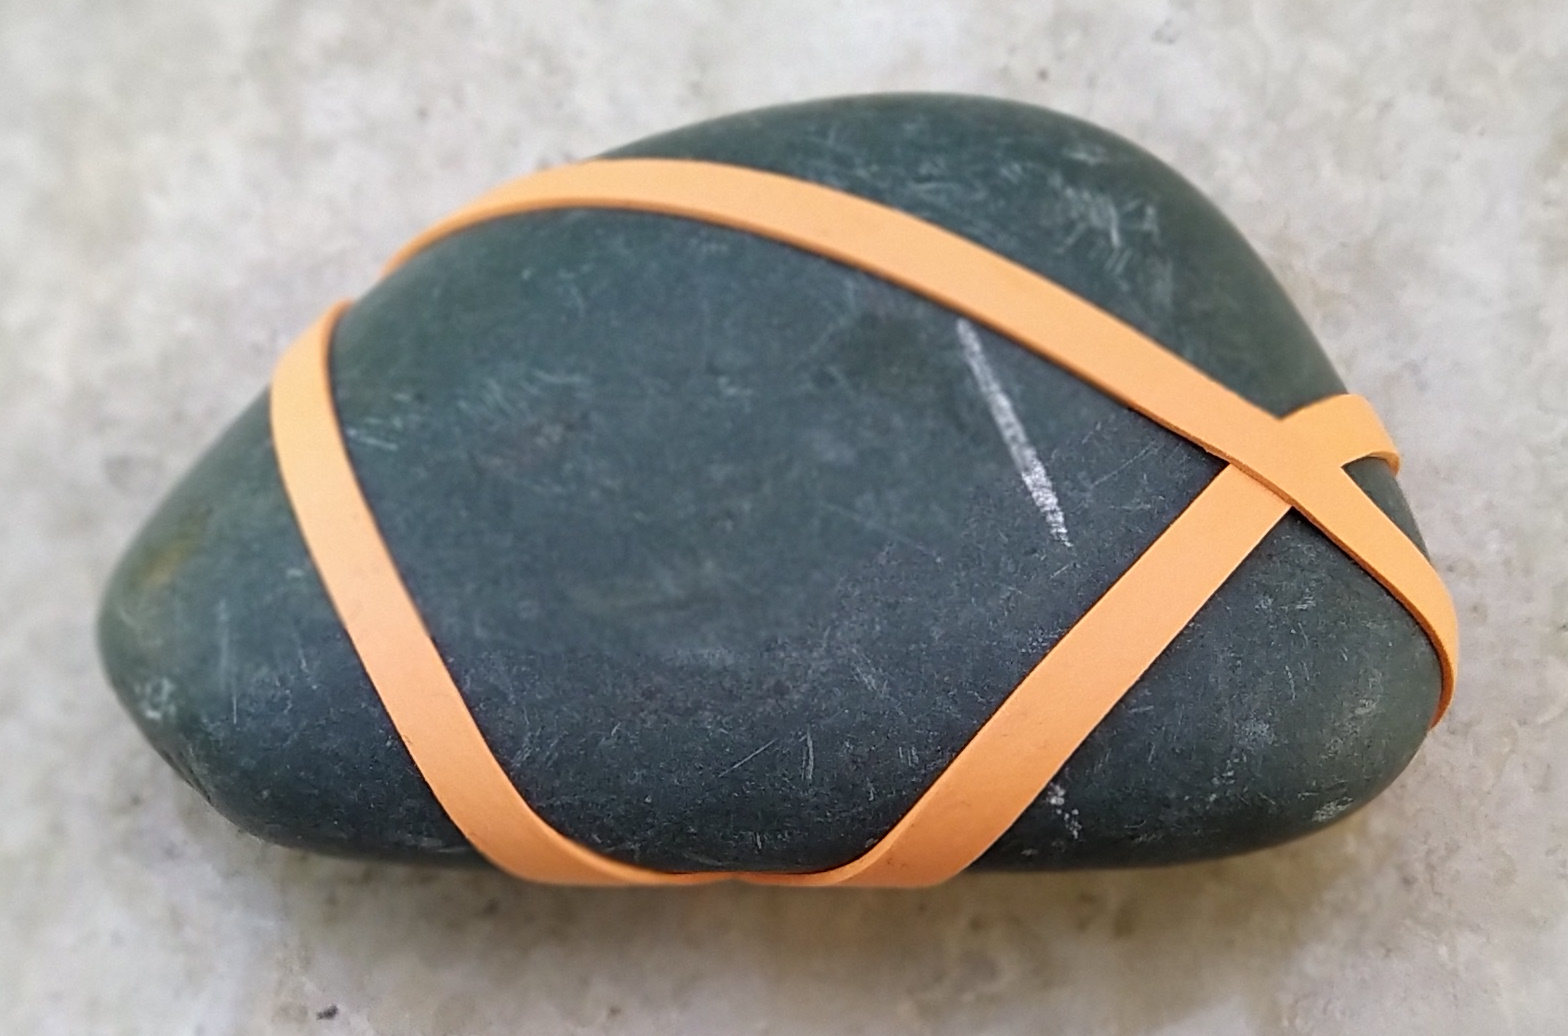
\includegraphics[width=\textwidth]{pics/pebble.jpg}
\end{minipage}
\hfill
\begin{minipage}{.30\textwidth}
\centering
\includegraphics{mppics/pic-50}
\end{minipage}
\hfill
\end{figure}
The combinatorics of self-crossings can be described by a closed plane curve --- it is the rubber band in a parametrization of the surface with one point removed.
For example, if you could turn the pebble around you would see that the self-crossings are described by the plane curve on the right diagram.

We assume that the surface of the pebble is strongly convex, smooth, and frictionless;
in this case, the rubber band models a closed geodesic.
Suppose that we are interested in possible patterns of self-crossings; more precisely:

\medskip

\emph{What are the possible combinatoric types of self-crossings of a closed geodesic on a strongly convex smooth closed surface?}

\begin{figure}[ht!]
\begin{center}
\includegraphics{mppics/pic-55}
\end{center}
\end{figure}

Consider the six possible patterns with three double crossings.
Configurations 1, 2, 3, and 4 can be realized as mirror-symmetric geodesics on mirror-symmetric surfaces; the projections on the plane of symmetry are sketched.
\begin{figure}[ht!]
\begin{center}
\includegraphics{mppics/pic-100}
\end{center}
\end{figure}

Further, we will discuss \emph{forbidden} configurations;
that is, configurations that cannot appear for closed geodesic.
These are configurations 5 and 6.

This question is a good exercise --- it could be explained to anyone, but an answer requires a considerable part of the theory.
The reader is welcome to try the cases with more self-crossings, but the general question seems to be hard;
I do not expect to see a complete classification in my lifetime.
Our question is closely related to the so-called \emph{flat knot types} of geodesics;
see \cite{angenent} and the references therein.

In what follows, we discuss the Gauss--Bonnet formula as well as the Alexandrov--Toponogov theorem and apply them to forbid configurations 5 and 6.
These theorems are covered in our textbook \cite{petrunin-zamora} which I like, altho they are treated in plenty of other places as well.


\section*{Gauss--Bonnet and no 5}

Suppose that $\Delta$ is an $n$-gon with geodesic sides in a surface $\Sigma$.
Recall that by the \emph{Gauss--Bonnet formula} the sum of the external angles of $\Delta$ equals
\[2\cdot\pi\cdot\chi(\Delta)-\int\limits_\Delta K,\]
where $\chi(\Delta)$ denotes the \emph{Euler characteristic} of $\Delta$ and $K$, the Gauss curvature of~$\Sigma$.

Further, we assume that $\Sigma$ is a closed strongly convex surface. In this case,
\begin{itemize}
 \item $\Sigma$ has strictly positive Gauss curvature;
 \item $\Sigma$ is homeomorphic to the sphere and therefore $\chi(\Sigma)=2$;
 \item %by Jordan--Schönflies theorem, 
 $\Delta$ is homeomorphic to the disc and therefore $\chi(\Delta)=1$.
\end{itemize}
It follows that the sum of the internal angles of $\Delta$ is lager than $(n\z-2)\cdot\pi$.
In particular, if $\Delta$ is a triangle with angles $\alpha$, $\beta$, and $\gamma$, then
\[\alpha+\beta+\gamma>\pi.\leqno({*})\]
The Gauss--Bonnet formula can be applied to the whole surface; it implies that
the integral of Gauss curvature along  $\Sigma$ is exactly $4\cdot\pi$.

{

\begin{wrapfigure}{r}{33 mm}
\vskip-8mm
\centering
\includegraphics{mppics/pic-3}
\end{wrapfigure}

\parit{No 5 is forbidden.}
Suppose there is a geodesic with self-crossings as on the diagram;
it divides the surface $\Sigma$ into one triangle, say $\Delta$, one hexagon, and three monogons.
Denote by $\alpha$, $\beta$, and $\gamma$ the internal angles of $\Delta$.

Note that three monogons have internal angles $\alpha$, $\beta$, and~$\gamma$.
By the Gauss--Bonnet formula, the integral of Gauss curvature along each monogon is 
$\pi\z+\alpha$, $\pi\z+\beta$, and $\pi\z+\gamma$ 
respectively.
By $({*})$ the integral of Gauss curvature along the three monogons exceeds $4\cdot \pi$.
But $4\cdot \pi$ is the integral of Gauss curvature along the \emph{whole} surface  --- a contradiction.

}

\section*{Alexandrov--Toponogov and no 6}

Let $\Delta$ be a geodesic triangle with angles $\alpha$, $\beta$, and $\gamma$ on the surface $\Sigma$.
Assume that the sides of $\Delta$ are length-minimizing among the curves \emph{in} $\Delta$ with the same endpoints, then the inequality $({*})$ can be made more exact.

Namely consider the so-called \emph{model triangle} $\tilde\Delta$ of $\Delta$; that is, $\tilde\Delta$ is a plane triangle with equal corresponding sides.
Since the sides are length-minimizing, they satisfy the triangle inequality; therefore the model triangle is defined.

Denote by $\tilde \alpha$, $\tilde \beta$ and $\tilde \gamma$ the angles of $\tilde\Delta$ respectively.
Then 
\[
\alpha> \tilde \alpha,
\qquad
\beta> \tilde \beta,
\qquad
\text{and}
\qquad
\gamma> \tilde \gamma.
\leqno({*}{*})
\]
Since $\tilde\alpha+\tilde\beta+\tilde\gamma=\pi$, this inequality implies $({*})$.

The inequality $({*}{*})$ easily follows from the proof of the \emph{Alexandrov--Toponogov theorem}.
The latter states that $({*}{*})$ holds for triangles with length-minimizing sides in the whole surface.
The proof is left as an 
exercise for those familiar with the Alexandrov--Toponogov theorem; other readers may simply accept it as true.

\parit{No 6 is forbidden.}
Suppose that the surface $\Sigma$ contains such a geodesic $\xi$;
assume that arcs and angles are labeled as in the leftmost part of the diagram below.
Applying the Gauss--Bonnet formula to the quadrangle and pentagon that the geodesic cuts from $\Sigma$, we get that
\[2\cdot\alpha<\beta+\gamma
\qquad\text{and} \qquad
2\cdot\beta+2\cdot \gamma<\pi+\alpha.\leqno(\asterism)\]
It follows that $\alpha <\tfrac \pi 3$.

\begin{figure}[!ht]
\vskip-1mm
\begin{minipage}{.22\textwidth}
\centering
\includegraphics{mppics/pic-472}
\end{minipage}
\hfill
\begin{minipage}{.35\textwidth}
\centering
\includegraphics{mppics/pic-473}
\end{minipage}
\hfill
\begin{minipage}{.35\textwidth}
\centering
\includegraphics{mppics/pic-474}
\end{minipage}
\vskip-1mm
\end{figure}

Consider the part of $\xi$ without the arc labeled by~$a$.
It cuts from $\Sigma$ a pentagon $\Delta$ with sides and angles shown in the middle part of the diagram.

Let us add additional vertices on the sides of $\Delta$ so that each side becomes length-minimizing.
Choose a vertex $v$ and subdivide $\Delta$ into triangles with minimizing sides by joining $v$ to other vertices.

Consider a model triangle for each triangle in the subdivision;
the model triangles lie in the plane and we suppose that they share sides as in $\Delta$.
By the comparison inequality $({*}{*})$, the angles of the model triangles do not exceed the corresponding angles of the original triangle.
Therefore the model triangles form a convex plane polygon, say $\tilde\Delta$.
Moreover, the five angles of $\tilde\Delta$ that correspond to the angles of $\Delta$ do not exceed those.

\begin{wrapfigure}{r}{50 mm}
\vskip-5mm
\centering
\includegraphics{mppics/pic-500}
\vskip-1mm
\end{wrapfigure}

It remains to show that the described plane polygon $\tilde\Delta$ does not exist.

Let us orient the sides of $\tilde\Delta$ counterclockwise;
denote the obtained vectors by $s_1,\dots,s_k$.
On one hand, the conditions on the angles of the polygons imply that the vectors $s_i$ point in the complement of white sectors shown with angles marked on the diagram.
The sum of the magnitudes of the vectors in each black sector is also marked.
Let $v$, $v'$, $w$, $w'$ be the marked unit vectors;
set $r=v+v'+w+w'$.
Observe that $(\asterism)$ implies that $r\ne 0$,
and, moreover, 
\[\langle r,s_1\rangle+\dots+\langle r,s_k\rangle>0.\]
On the other hand, the vectors $s_i$ circumambulate a polygon; therefore, 
\[s_1+\dots+s_k=0\]
--- a contradiction.

{\small \parbf{Acknowledgments.}
I want to thank Sergio Zamora Barrera for help.
This work was supported by the NSF, grant DMS-2005279 and Simons Foundation, grant \#584781.}



{\sloppy
\printbibliography
\fussy
}

\end{document}
